\documentclass{VUMIFPSkursinis}
\usepackage{algorithmicx}
\usepackage{algorithm}
\usepackage{algpseudocode}
\usepackage{amsfonts}
\usepackage{amsmath}
\usepackage{bm}
\usepackage{caption}
\usepackage{color}
\usepackage{float}
\usepackage{graphicx}
\usepackage{listings}
\usepackage{subfig}
\usepackage{array}
\usepackage{wrapfig}
\usepackage{tabu}

% Titulinio aprašas
\university{Vilniaus universitetas}
\faculty{Matematikos ir informatikos fakultetas}
\department{Programų sistemų katedra}
\papertype{Kursinis darbas}
\title{Blokų grandinių duomenų bazės finansinių duomenų kaupimui}
\titleineng{Blockchain databases for financial data}
\status{3 kurso 3 grupės studentas}
\author{Matas Savickis}
% \secondauthor{Vardonis Pavardonis}   % Pridėti antrą autorių
\supervisor{dr. Vytautas Valaitis}
\date{Vilnius – \the\year}

% Nustatymai
% \setmainfont{Palemonas}   % Pakeisti teksto šriftą į Palemonas (turi būti įdiegtas sistemoje)
\bibliography{bibliografija}

\begin{document}
\maketitle

\tableofcontents

\sectionnonum{Įvadas}
Per pastaruosius keletą metų blokų grandinių technologija susilaukė didelio žmonių susidomėjimo. 
Šis susidomėjimas daugiausiai kilo dėl išpopulerėjusių kriptovaliutų, tokių kaip Bitcoin, Etherium, Litecoin ir daugeliu kitų 
kurios ir yra paremtos blokų grandinių technologija. Šią technologiją 2008 metais sukūrė Satošis Nakamoto  \cite{BlockChain}. 
2009 metais Nakamoto implementavo blokų grandinių technologiją sukurdamas Bitcoin kriptovaliutą \cite{Bitcoin}. 
Nors, šiuo metu, žmonių susidomėjimas kripto valiutomis ir yra sumažėjęs \cite{Trends}, tačiau informacinių technologijų industrija 
mato daugiau blokų grandinių panaudojimo atveju negu tik kripto valiutos. Vienas iš blokų grandinių panaudojimo atvėjų yra 
blokų grandinių duomenų bazės. Reliacinės ir dokumentų duomenų bazės ilgą laiką buvo pagrindinis duomenų saugojimo būdas. 
Tačiau šios duomenų bazės turi ir savo trūkumų, saugant duomenis tradicinėsė duomenų bazėse kyla duomenų integralumo problemos \cite{Integrity}
. 
Naudojant duomenų bazes financinėms transakcijoms sekti kyla dvigumo pinigų išleidimo problema\cite{Double}
. Naudojantis tradicinėmis duomenų bazėmis 
taip pat kyla pasitikėjimo problema, visa duomenų prieeiga yra trečiosios šalies valdžioje, ir vartotojas turi pasitikėti, kad duomenys nebus pakeisti be jo žinios.
Per pastaruosius kelis metus šias problemas
 buvo stengtasi išspręsti kuriant duomenų bazes paremtas blokų grandinių technologija. Privačios blokų grandinių duomenų bazės užtikrina pasitikėjimą, nes kiekvienas vartotojas turi visą duomenų 
bazės kopiją. Darant pakeitimus tokioje duomenų bazėje kiekvienas vartotojas turi sutikti su daromais pakeitimais ir saugo visų pakeitimų istoriją. Blokų grandinių duomenų bazės išsprendžia duomenų integralumo ir
dvigumo pinigų išleidimo problemą, nes kiekvienas mazgas blokų grandinėje tinkle gali palyginti savo turimus duomenis su kitais mazgais. 
Nors blokų grandinės išsprendžia autoriaus išvardytas problemas, tačiau finansinėms transakcijos svarbus ir greitis. Šiuo darbu siekia atlikti blokų grandinių duomenų bazių analizę greičio aspektu.

\sectionnonum{Uždaviniai}
	\begin{enumerate}
		\item{Palyginti Cassandra NoSQL transakcijų praeinamumo greičius su Hyperledger Fabric blokų grandinių duomenų baze}
		\item{Palyginti Cassandra NoSQL transakcijų vėlavimą su Hyperledger Fabric blokų grandinių duomenų bazėmis}
		\item{Išskirti esamų tyrimų trūkumus ir galimas sritis ateities darbams}
		
		
	\end{enumerate}
\pagebreak
\section{Literatūros analizė}
	\subsection{Hyperledger}
		Hyperleadger yra atviro kodo blokų grandinės pradėtos pradėtos kurti Linux fondo. Šio projekto tikslas yra gerinti tarpindustrini bendradarbiavimą kuriant blokų grandines kurios užtikrintų 
		patikimą, greitą ir saugų finansinių duomenų perdavimą pagrindinėse technologijų, finansų ir produktų tiekimo kompanijose \cite{LinuxHyper}. Šiame skirsnyje bus apžvelgti 
		Hyperledger Fabric, populiariausios Hyperledger implementacijos, architektūra, greičio tyrimai, kaip šie tyrimai buvo atlikti, kokie parametrai įtakoja Hyperledger greitį ir pateikta tolimesnės analizės pasiūlymai. 
		
		\subsubsection{Architektūra}
			Hyperledger Fabric(toliau - Fabric) yra privati blokų grandinė skirta įmonių lygio aplikacijoms. 
			Ši blokų grandinė gali vykdyti arbitrišką išmanujį kontraktą parašyta Java, Go arba NodeJS kalbomis (grandinės kodai).
			Fabric sudaro šios esybės:
			\begin{itemize}
				\item{Lygiarangis - šis mazgas yra atsakingas už grandinės kodą kurį vykdant yra įgyvendinamas išmanusis kontraktas. 
 Lygiarangis savyje turi visą tinklo informaciją(angl. Ledger). }
				\item{Užsakymo servisas (angl. Ordering Service) - Užsakymo serviso mazgas dalyvauja susitarimo(angl. consensus) 
protokole ir padalina bloką taip, kad jį būtų galima naudoti tranzakcijom. Padalintas blokas būna persiunčiamas kitiems lygiarangiams.}
				\item{Klientas - atsakingas už transakcijos siūlymo sukūrimą, ir išsiuntimą tinklo lygiarangiams. Gavus patvirtinimą iš lygiarangių vartotojas siunčia prašymą tvarkytojui, kad jis informaciją įtrauktų į bloką ir išsiūstų ją visiems tinklo perams.}
			\end{itemize}

		\subsubsection{Tranzakcijų vykdymas}

			Tranzakcijos vyksta trejomis fazėmis(1 pav.):
			\begin{enumerate}
				\item{Patvirtinimo fazė - simuliuojama tranzakcija su pasirinktais vienarangiais ir renkami būsenos pokyčiai}
				\item{Užsakymo fazė - užsakomos tranzakcijos per susitarimo protokolą}
				\item{Patvirtinimo fazė - patvirtinimas ir informacijos įdėjimas į buhalterinę knygą }
			\end{enumerate}

\begin{figure}[H]
    \centering
    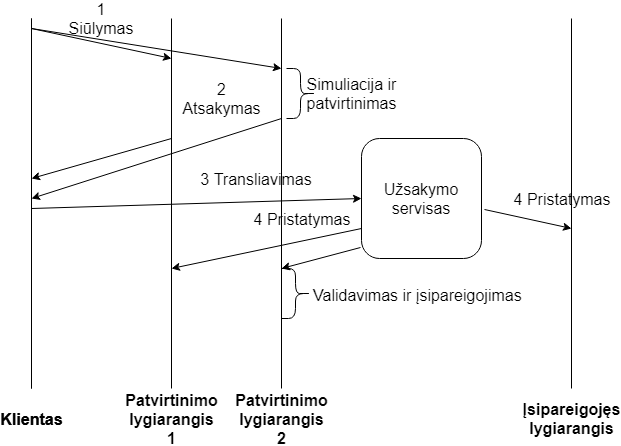
\includegraphics[scale=0.5]{img/MLP}
    \caption{Tranzakcijų sekų diagrama}   % Antraštė įterpiama po paveikslėlio
    \label{img:mlp}
\end{figure}



				
		\subsubsection{Parametrai}

Yra grupė parametrų \cite{IMBResearch} kurie įtakoja Fabric greitį 
			
			\begin{itemize}
				\item{Mazgų skaičius - vartotojų skaičius privačioje blokų grandinėje}
				\item{Tranzakcijų skaičius - keičiant tranzakcijų skaičiū keičiasi vėlavimas ir pralaidumas}
				\item{Bloko dydis - tranzakcijos yra sugrupuojamos į blokus. Blokai yra siunčiami visiems tinklo perams. Užsakymo parašas 
būna verifikuojamas kiekvienam blokui, o perdavimo patvirtinimo parašas verifikuojamas kiekvienai transakcijai, todėl keičiant bloko dydį atsiranda kompropisas tarp palaidumo ir vėlavim}
				\item{Patvirtinimo politika - diktuoja kiek tranzakcijų ir pasirašymų turi būti įvykdyta prieš siunčiant tranzakcijas užsakytoją. Didinant politikos sudėtingumą didės resursų sunaudojimas ir įvertinimo laikas.}
				\item{Kanalai - izoliuoja tranzakcijas viena nuo kitos ir norint persiųsti tranzakcijas iš vieno kanalo į kitą turi būti patvirtintos, surikiuotos ir apdorotos nepriklausomai viena nuo kitos.}
				\item{Resursų paskirstymas - kiekvienas lygiarangis vykdo grandinės kodą skirtą parašo skaičiavimams ir verifikavimo rutinoms. Keičiant procesoriaus branduolių skaičių keičiasi vykdymo greitis.}
				\item{Būsenos duomenų bazė - Fabric naudoją dvi duomenų bazes, CouchDB ir GoLevelDB, kuriuose galima saugoti ledgerio buseną}
			\end{itemize}

		\subsubsection{Testavimo metodologijos}
			Šiame darbe apžvelgta trijų straipsnių duomenys, juose naudota tokia kompiuterinė įranga:
\begin{center}
\begin{tabular}{ | m{5em} | m{10cm}| } 
\hline
\cite{IMBResearch}& x86 64 virtuali mašina IBM SoftLayer duomenų centre. 
Kiekvienai virtualiai mašinai yra alokuota 32 vCPUs  Intel(R) Xeon(R)
CPU E5-2683 v3 @ 2.00GHz ir 32 GB atminties. Trys kliento mašinos skirtos generuoti apkrovą buvo alokuota
 56 vCPU ir 128 GB RAM. Mazgai prijungti prie 3 Gbps duomenų centro tinklo  \\ 
\hline
 \cite{ThailandPerf}& Amazon AWS EC2
 su Intel E5-1650 8 branduolių CPU,
15GB RAM, 128GB SSD  \\ 
\hline
 \cite{ShaFabPerf}& HPC serveris
su Intel(R) Xeon(R) CPU E5-2690, 2.60 GHz, 24 core
CPU, 64 GB RAM, and running Ubuntu 16.04  \\ 
\hline
\end{tabular}
\end{center}

		\subsubsection{Tyrimų rezultatai}
\begin{figure}[H]
    \centering
    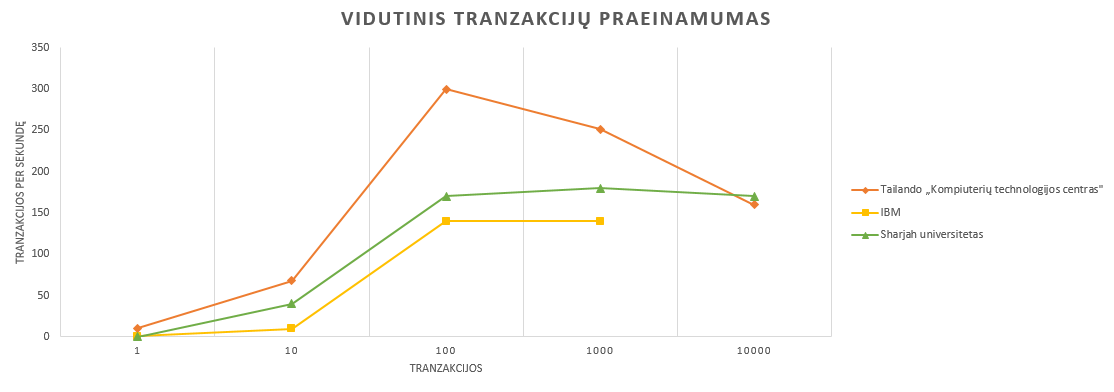
\includegraphics[scale=0.5]{img/Praein}
    \caption{Tranzakcijų praeinamumas}   % Antraštė įterpiama po paveikslėlio
    \label{img:mlp}
\end{figure}		
\begin{figure}[H]
    \centering
    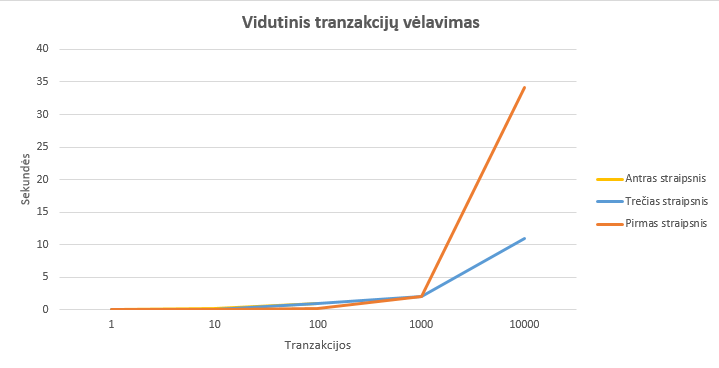
\includegraphics[scale=0.5]{img/Velav}
    \caption{Tranzakcijų vėlavimas}   % Antraštė įterpiama po paveikslėlio
    \label{img:mlp}
\end{figure}		

		\subsubsubsection{IBM tyrimas}
			IBM atliktame tyrime \cite{IMBResearch} buvo tyriama kaip keičiant Fabric parametrus keičiasi tranzakcijų praeinamumas ir vėlavimas. Didinant tranzakcijų atvykimo kiekį nuo 20 tranzakcijų per sekundę iki 100 praeinamumas dideja tiesiškai, o nuo 100 transakcijų per sekundę praeinamumas sustojo ir nebekilo. Bloko dydis praeinamumui įtakos neturėjo. 
\newline
Mažiausias vėlavimas būna pasirinkus mažiausia bloko dydį. Keičiant tranzakcijų atvykimo kiekį nuo 25 iki 125 vėlavimas išlieka apie 0,3 sekundės ir tuomet smarkiai kyla iki 10 sekundžių tranzakcijų 
atvykimo kiekį pakėlus iki 150 transakcijų. 
\newline
Iš šio tyrimo imsime geriausius rezultatus(2 pav. ir 3 pav.) ir vėliau lyginsime juos su MySQL ir PostgreSQL duomenų bazėmis. 
		\subsubsubsection{Tailando ,,Kompiuterių technologijos centro" tyrimas}
			Tailando ,,Kompiuterių technologijos centro" atliktame darbe buvo simuliuojamos pinigų siuntimas, pinigų išdavimas ir vartotojų sukūrimas. Keliant tranzakcijų skaičių iki 100 praeinamumas kilo iki 299.85 tranzakcijų per sekundę. Didinant tranzakcijų kaičių iki 1000 praeinamumas pakito nežymiai, kaip ir IBM \cite{IMBResearch} atliktame darbe, ir didinant tranzakcijų skaičių iki 10000 praeinamumas krito iki 159.76 tranzakcijų per sekundę. 
Didinant tranzakcijas nuo 1 iki 100 vėlavimas kilo nežymiai, nuo 0.09 iki 0.17. Padidinuos tranzakcijas nuo 100 iki 10000 staiga pakilo vėlavimas net iki 34.08 sekundžių.
		\subsubsubsection{Sharjah tyrimas}
			Sharjah universiteto mokslininkų tyrime \cite{ShaFabPerf} Fabric 0.6 ir Fabric 1.0 tranzakcijų praeinamumas ir vėlavimas. Nuo 10 iki 100 tranzakcijų praeinamumas kilo nuo 40 tranzakcijų per sekundę iki 165 tranzakcijų per sekundę, toliau didinant tranzakcijų skaičių praeinamumas nebekito. Toks rezultatas gautas naudojant Fabric 1.0 versija ir praeinamumas geresnis negu Fabric 0.6 versijos. 
Didinant tranzakcijų skaičių nuo 10 iki 1000 vėlavimas pakilo nežymiai, nuo 0.1 sekundės iki 1 sekundės, tačiau padidinus tranzakcijų skaičių iki 10000 pastebėtas didelis vėlavimo pašokimas iki 10 sekundžių.
Šio darbo metodologija buvo paremta jau minėtu Tailando mokslininkų darbu \cite{ThailandPerf}

\subsubsubsection{Rezultatu apibendrinimas}
Iš aukščiau aptartų darbų(\cite{IMBResearch}, \cite{ThailandPerf}, \cite{ShaFabPerf}) pastebima tendencija, kad didinant tranzakcijų skaičių iki 100 praeinamumas kilo tiesiškai, o didinant transakcijų skaičių toliau praeinamumas nebekilo arba net krito(\cite{ThailandPerf}).
\newline
Didinant tranzakcijas nuo 1 iki 1000 vėlavimas praktiškai nekyla, ir tada nuo 1000 iki 10000 vėlavimas smarkiai šoktelėja. 
									


			

	\subsection{MySQL ir PostgreSQL}

\section{Išvados}

\section{Priedai}
\subsection{Žodynas}
\begin{itemize}
	\item{Grandinės kodas(angl. chaincode) - programa parašyta Go, Java arba NodeJS kalbomis kuri vykdo
 verslo logiką sutartą tarp tinklo narių.}
	\item{Lygiarangis(angl. peer) - tinklo dalyvis gaunantis ir siunčiantis informaciją.}
	\item{Išmanusis kontraktas(smart contract)}
\end{itemize}


\printbibliography[heading=bibintoc]  









\end{document}
